\documentclass[a4paper,12pt]{report}

\usepackage[utf8]{inputenc}
\usepackage{amsmath}
\usepackage{graphicx}
\usepackage{hyperref}
\usepackage{geometry}
\usepackage[labelfont=bf]{caption}
\usepackage{caption}
\usepackage{subcaption}
\geometry{a4paper, margin=1in}

\begin{document}

\begin{titlepage}
    \centering
    {\large\bfseries RANCANG BANGUN SISTEM PEMBELIAN TIKET PESAWAT BERBASIS APLIKASI DESKTOP GUI DENGAN BAHASA C DAN DATABASE MYSQL\par}
    \vspace{0.3cm}
    {\large\bfseries PROJECT AKHIR\par}
    {\large\bfseries PRAKTIKUM DASAR PEMROGRAMAN\par}
    \vspace{2cm}
    \vspace*{0.5cm}
    
\includegraphics[width=0.4\textwidth]{Logo_PENS.png}\par\vspace{1cm}
    \vspace{1cm}
    {\large\bfseries Dosen :\par}
    {\Large\itshape Norma Ningsih, S.ST., M.T.\par}
    \vspace{1cm}
    {\large\bfseries Oleh :\par}
    {\Large\itshape Muqsith Barru Pamungkas - 2423600035\\Riski Gana Prasetya - 2423600053\par}
    \vspace{1cm}
    {\scshape\LARGE Teknologi Rekayasa Internet \par}
    {\scshape\LARGE Departemen Teknik Elektro \par}
    \vspace{0.5cm}
    {\scshape\Large POLITEKNIK ELEKTRONIKA NEGERI SURABAYA\par}
    {\scshape\Large 2024\par}
    \vfill
\end{titlepage}

% \title{RANCANG BANGUN SISTEM PEMBELIAN TIKET PESAWAT BERBASIS APLIKASI DESKTOP GUI DENGAN BAHASA C DAN MYSQL}
% \author{{Muqsith Barru Pamungkas}\and
% \date{\today}
% {Riski Gana Prasetya}}
% \begin{document}
% \begin{abstract}
% Makalah ini memberikan contoh sederhana bagaimana membuat dokumen menggunakan LaTeX. Kami mencakup elemen-elemen dasar seperti judul, penulis, abstrak, pendahuluan, dan kesimpulan. LaTeX adalah alat yang sangat berguna untuk penulisan dokumen ilmiah karena kemampuannya untuk mengatur format secara otomatis.
% \end{abstract}

\section{Pendahuluan}
\label{sec:intro}

LaTeX adalah sistem penyiapan dokumen berkualitas tinggi. Sistem ini sering digunakan untuk dokumen teknis atau ilmiah, termasuk makalah, buku, dan presentasi. LaTeX memungkinkan penulis untuk fokus pada konten dokumen tanpa harus khawatir tentang format.

\section{Metode}

Dalam bagian ini, kita menjelaskan metode yang digunakan untuk menulis makalah ini. Penulis dapat menggunakan berbagai paket dan perintah LaTeX untuk menyusun dokumen yang rapi dan terorganisir.

\subsection{Paket-paket LaTeX}
Beberapa paket yang digunakan dalam dokumen ini meliputi:
\begin{itemize}
    \item \texttt{inputenc} untuk pengkodean karakter.
    \item \texttt{amsmath} untuk menulis rumus matematika.
    \item \texttt{graphicx} untuk menyisipkan gambar.
    \item \texttt{hyperref} untuk membuat hyperlink.
    \item \texttt{geometry} untuk mengatur margin halaman.
\end{itemize}

\section{Hasil dan Pembahasan}

LaTeX sangat berguna untuk menulis rumus matematika dan menyisipkan gambar. Berikut adalah contoh rumus matematika:
\begin{equation}
E = mc^2
\end{equation}

Dan berikut adalah contoh gambar yang disisipkan:
\begin{figure}[h]
    \centering
    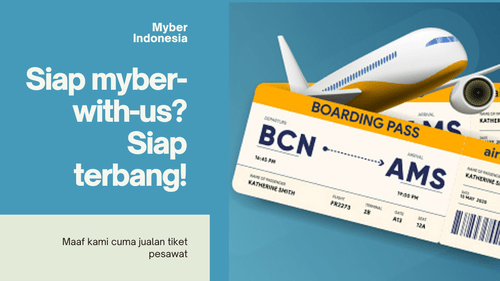
\includegraphics[width=0.5\textwidth]{../assets/banner.png}
    \caption{Contoh gambar}
    \label{fig:example}
\end{figure}



\section{Kesimpulan}
LaTeX adalah alat yang sangat berguna untuk menulis dokumen ilmiah. Dengan menggunakan LaTeX, penulis dapat dengan mudah mengatur format dokumen dan fokus pada konten.

\section*{Referensi}
\begin{itemize}
    \item Lamport, L. (1994). \textit{LaTeX: A Document Preparation System}. Addison-Wesley.
    \item \url{https://www.latex-project.org/}
\end{itemize}

\end{document}
